\section{Измерение продольной поляризации $\Lambda_c \to \Lambda \pi$}

С помощью формализма спиральных амплитуд \textbf{\cite{Richman}} можно описать процесс 
$\Lambda_c \to \Lambda \pi$ и получить его угловое распределение с 
учётом продольной поляризации. На рис. \ref{def:val} показаны определения 
наблюдаемых величин. 

\begin{figure}[H]
    \centering
    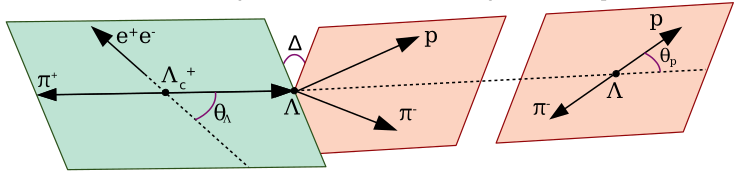
\includegraphics[width=0.7\linewidth]{img/lpi_def.png}
    \caption{Определение переменных.}
    \label{def:val}
\end{figure}

Амплитуда записывается следующим образом:

\begin{equation}
    A_{\llp{c} \llp{p}} = \sum_{\llp{c}} A_{\llp{c}} D^{1/2\dag}_{\llp{c} \llp{p}}\left(\phi_\lambda, \theta_\Lambda, -\phi_\Lambda \right) D^{1/2\dag}_{\llp{c} \llp{p}} B_{\llp{p}} D^{1/2}_{\llp{c} \llp{p}}\left(\phi_\lambda, \theta_\Lambda, -\phi_\Lambda \right)
\end{equation}

Где $\llp{p}$ --- спиральность протона, 
$A_{\llp{c}}$ --- спиральная амплитуда $\Lambda_c \to \Lambda \pi^+$, 
$B_{\llp{c}}$ --- спиральная амплитуда $\Lambda_c \to \Lambda \pi^-$,



